% Graphic for TeX using PGF
% Title: /home/marta/Documentos/Git/TFG/clases.dia
% Creator: Dia v0.97.3
% CreationDate: Fri Oct 21 13:35:53 2016
% For: marta
% \usepackage{tikz}
% The following commands are not supported in PSTricks at present
% We define them conditionally, so when they are implemented,
% this pgf file will use them.
\ifx\du\undefined
  \newlength{\du}
\fi
\setlength{\du}{15\unitlength}
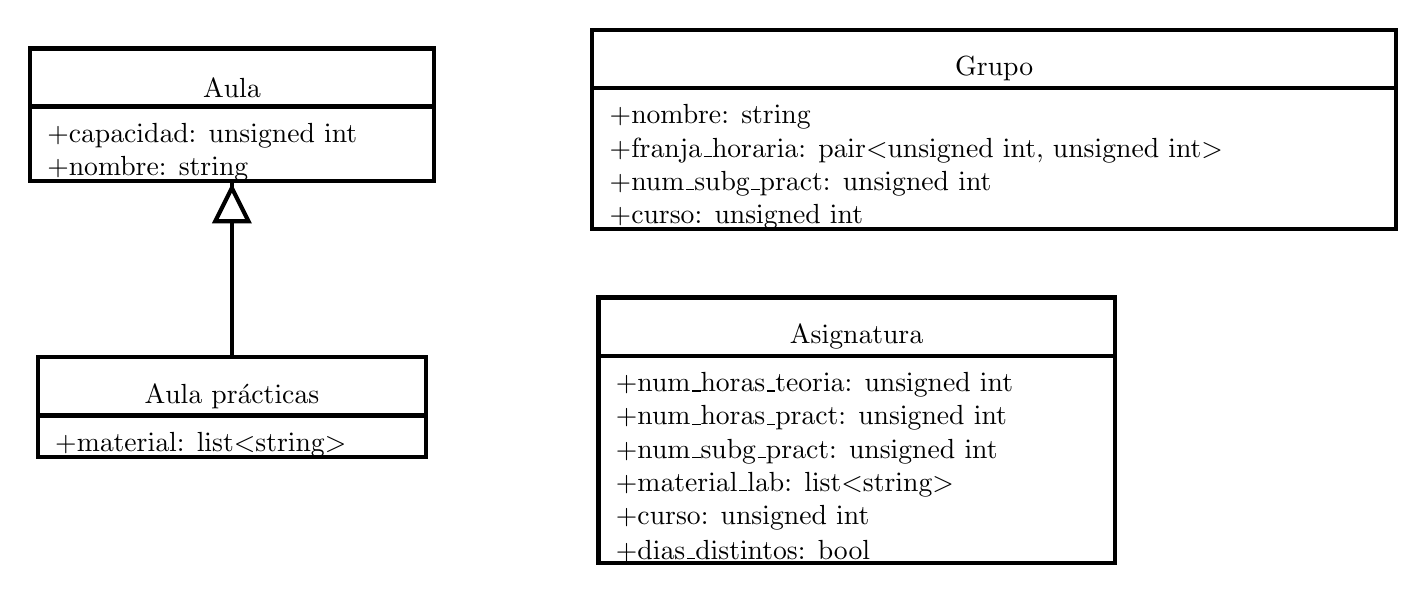
\begin{tikzpicture}
\pgftransformxscale{1.000000}
\pgftransformyscale{-1.000000}
\definecolor{dialinecolor}{rgb}{0.000000, 0.000000, 0.000000}
\pgfsetstrokecolor{dialinecolor}
\definecolor{dialinecolor}{rgb}{1.000000, 1.000000, 1.000000}
\pgfsetfillcolor{dialinecolor}
\pgfsetlinewidth{0.100000\du}
\pgfsetdash{}{0pt}
\definecolor{dialinecolor}{rgb}{1.000000, 1.000000, 1.000000}
\pgfsetfillcolor{dialinecolor}
\fill (14.350000\du,6.150000\du)--(14.350000\du,7.550000\du)--(24.090000\du,7.550000\du)--(24.090000\du,6.150000\du)--cycle;
\definecolor{dialinecolor}{rgb}{0.000000, 0.000000, 0.000000}
\pgfsetstrokecolor{dialinecolor}
\draw (14.350000\du,6.150000\du)--(14.350000\du,7.550000\du)--(24.090000\du,7.550000\du)--(24.090000\du,6.150000\du)--cycle;
% setfont left to latex
\definecolor{dialinecolor}{rgb}{0.000000, 0.000000, 0.000000}
\pgfsetstrokecolor{dialinecolor}
\node at (19.220000\du,7.100000\du){Aula};
\definecolor{dialinecolor}{rgb}{1.000000, 1.000000, 1.000000}
\pgfsetfillcolor{dialinecolor}
\fill (14.350000\du,7.550000\du)--(14.350000\du,9.350000\du)--(24.090000\du,9.350000\du)--(24.090000\du,7.550000\du)--cycle;
\definecolor{dialinecolor}{rgb}{0.000000, 0.000000, 0.000000}
\pgfsetstrokecolor{dialinecolor}
\draw (14.350000\du,7.550000\du)--(14.350000\du,9.350000\du)--(24.090000\du,9.350000\du)--(24.090000\du,7.550000\du)--cycle;
% setfont left to latex
\definecolor{dialinecolor}{rgb}{0.000000, 0.000000, 0.000000}
\pgfsetstrokecolor{dialinecolor}
\node[anchor=west] at (14.500000\du,8.250000\du){+capacidad: unsigned int};
% setfont left to latex
\definecolor{dialinecolor}{rgb}{0.000000, 0.000000, 0.000000}
\pgfsetstrokecolor{dialinecolor}
\node[anchor=west] at (14.500000\du,9.050000\du){+nombre: string};
\pgfsetlinewidth{0.100000\du}
\pgfsetdash{}{0pt}
\definecolor{dialinecolor}{rgb}{1.000000, 1.000000, 1.000000}
\pgfsetfillcolor{dialinecolor}
\fill (14.542045\du,13.592045\du)--(14.542045\du,14.992045\du)--(23.897045\du,14.992045\du)--(23.897045\du,13.592045\du)--cycle;
\definecolor{dialinecolor}{rgb}{0.000000, 0.000000, 0.000000}
\pgfsetstrokecolor{dialinecolor}
\draw (14.542045\du,13.592045\du)--(14.542045\du,14.992045\du)--(23.897045\du,14.992045\du)--(23.897045\du,13.592045\du)--cycle;
% setfont left to latex
\definecolor{dialinecolor}{rgb}{0.000000, 0.000000, 0.000000}
\pgfsetstrokecolor{dialinecolor}
\node at (19.219545\du,14.542045\du){Aula prácticas};
\definecolor{dialinecolor}{rgb}{1.000000, 1.000000, 1.000000}
\pgfsetfillcolor{dialinecolor}
\fill (14.542045\du,14.992045\du)--(14.542045\du,15.992045\du)--(23.897045\du,15.992045\du)--(23.897045\du,14.992045\du)--cycle;
\definecolor{dialinecolor}{rgb}{0.000000, 0.000000, 0.000000}
\pgfsetstrokecolor{dialinecolor}
\draw (14.542045\du,14.992045\du)--(14.542045\du,15.992045\du)--(23.897045\du,15.992045\du)--(23.897045\du,14.992045\du)--cycle;
% setfont left to latex
\definecolor{dialinecolor}{rgb}{0.000000, 0.000000, 0.000000}
\pgfsetstrokecolor{dialinecolor}
\node[anchor=west] at (14.692045\du,15.692045\du){+material: list$<$string$>$};
\pgfsetlinewidth{0.100000\du}
\pgfsetdash{}{0pt}
\pgfsetmiterjoin
\pgfsetbuttcap
{
\definecolor{dialinecolor}{rgb}{0.000000, 0.000000, 0.000000}
\pgfsetfillcolor{dialinecolor}
% was here!!!
\definecolor{dialinecolor}{rgb}{0.000000, 0.000000, 0.000000}
\pgfsetstrokecolor{dialinecolor}
\draw (19.220000\du,9.400403\du)--(19.220000\du,11.871071\du)--(19.219545\du,11.871071\du)--(19.219545\du,13.541740\du);
}
\definecolor{dialinecolor}{rgb}{0.000000, 0.000000, 0.000000}
\pgfsetstrokecolor{dialinecolor}
\draw (19.220000\du,10.312206\du)--(19.220000\du,11.871071\du)--(19.219545\du,11.871071\du)--(19.219545\du,13.541740\du);
\pgfsetmiterjoin
\definecolor{dialinecolor}{rgb}{1.000000, 1.000000, 1.000000}
\pgfsetfillcolor{dialinecolor}
\fill (19.620000\du,10.312206\du)--(19.220000\du,9.512206\du)--(18.820000\du,10.312206\du)--cycle;
\pgfsetlinewidth{0.100000\du}
\pgfsetdash{}{0pt}
\pgfsetmiterjoin
\definecolor{dialinecolor}{rgb}{0.000000, 0.000000, 0.000000}
\pgfsetstrokecolor{dialinecolor}
\draw (19.620000\du,10.312206\du)--(19.220000\du,9.512206\du)--(18.820000\du,10.312206\du)--cycle;
% setfont left to latex
\pgfsetlinewidth{0.100000\du}
\pgfsetdash{}{0pt}
\definecolor{dialinecolor}{rgb}{1.000000, 1.000000, 1.000000}
\pgfsetfillcolor{dialinecolor}
\fill (27.900000\du,5.700000\du)--(27.900000\du,7.100000\du)--(47.265000\du,7.100000\du)--(47.265000\du,5.700000\du)--cycle;
\definecolor{dialinecolor}{rgb}{0.000000, 0.000000, 0.000000}
\pgfsetstrokecolor{dialinecolor}
\draw (27.900000\du,5.700000\du)--(27.900000\du,7.100000\du)--(47.265000\du,7.100000\du)--(47.265000\du,5.700000\du)--cycle;
% setfont left to latex
\definecolor{dialinecolor}{rgb}{0.000000, 0.000000, 0.000000}
\pgfsetstrokecolor{dialinecolor}
\node at (37.582500\du,6.650000\du){Grupo};
\definecolor{dialinecolor}{rgb}{1.000000, 1.000000, 1.000000}
\pgfsetfillcolor{dialinecolor}
\fill (27.900000\du,7.100000\du)--(27.900000\du,10.500000\du)--(47.265000\du,10.500000\du)--(47.265000\du,7.100000\du)--cycle;
\definecolor{dialinecolor}{rgb}{0.000000, 0.000000, 0.000000}
\pgfsetstrokecolor{dialinecolor}
\draw (27.900000\du,7.100000\du)--(27.900000\du,10.500000\du)--(47.265000\du,10.500000\du)--(47.265000\du,7.100000\du)--cycle;
% setfont left to latex
\definecolor{dialinecolor}{rgb}{0.000000, 0.000000, 0.000000}
\pgfsetstrokecolor{dialinecolor}
\node[anchor=west] at (28.050000\du,7.800000\du){+nombre: string};
% setfont left to latex
\definecolor{dialinecolor}{rgb}{0.000000, 0.000000, 0.000000}
\pgfsetstrokecolor{dialinecolor}
\node[anchor=west] at (28.050000\du,8.600000\du){+franja\_horaria: pair$<$unsigned int, unsigned int$>$};
% setfont left to latex
\definecolor{dialinecolor}{rgb}{0.000000, 0.000000, 0.000000}
\pgfsetstrokecolor{dialinecolor}
\node[anchor=west] at (28.050000\du,9.400000\du){+num\_subg\_pract: unsigned int};
% setfont left to latex
\definecolor{dialinecolor}{rgb}{0.000000, 0.000000, 0.000000}
\pgfsetstrokecolor{dialinecolor}
\node[anchor=west] at (28.050000\du,10.200000\du){+curso: unsigned int};
\pgfsetlinewidth{0.100000\du}
\pgfsetdash{}{0pt}
\definecolor{dialinecolor}{rgb}{1.000000, 1.000000, 1.000000}
\pgfsetfillcolor{dialinecolor}
\fill (28.050000\du,12.150000\du)--(28.050000\du,13.550000\du)--(40.485000\du,13.550000\du)--(40.485000\du,12.150000\du)--cycle;
\definecolor{dialinecolor}{rgb}{0.000000, 0.000000, 0.000000}
\pgfsetstrokecolor{dialinecolor}
\draw (28.050000\du,12.150000\du)--(28.050000\du,13.550000\du)--(40.485000\du,13.550000\du)--(40.485000\du,12.150000\du)--cycle;
% setfont left to latex
\definecolor{dialinecolor}{rgb}{0.000000, 0.000000, 0.000000}
\pgfsetstrokecolor{dialinecolor}
\node at (34.267500\du,13.100000\du){Asignatura};
\definecolor{dialinecolor}{rgb}{1.000000, 1.000000, 1.000000}
\pgfsetfillcolor{dialinecolor}
\fill (28.050000\du,13.550000\du)--(28.050000\du,18.550000\du)--(40.485000\du,18.550000\du)--(40.485000\du,13.550000\du)--cycle;
\definecolor{dialinecolor}{rgb}{0.000000, 0.000000, 0.000000}
\pgfsetstrokecolor{dialinecolor}
\draw (28.050000\du,13.550000\du)--(28.050000\du,18.550000\du)--(40.485000\du,18.550000\du)--(40.485000\du,13.550000\du)--cycle;
% setfont left to latex
\definecolor{dialinecolor}{rgb}{0.000000, 0.000000, 0.000000}
\pgfsetstrokecolor{dialinecolor}
\node[anchor=west] at (28.200000\du,14.250000\du){+num\_horas\_teoria: unsigned int};
% setfont left to latex
\definecolor{dialinecolor}{rgb}{0.000000, 0.000000, 0.000000}
\pgfsetstrokecolor{dialinecolor}
\node[anchor=west] at (28.200000\du,15.050000\du){+num\_horas\_pract: unsigned int};
% setfont left to latex
\definecolor{dialinecolor}{rgb}{0.000000, 0.000000, 0.000000}
\pgfsetstrokecolor{dialinecolor}
\node[anchor=west] at (28.200000\du,15.850000\du){+num\_subg\_pract: unsigned int};
% setfont left to latex
\definecolor{dialinecolor}{rgb}{0.000000, 0.000000, 0.000000}
\pgfsetstrokecolor{dialinecolor}
\node[anchor=west] at (28.200000\du,16.650000\du){+material\_lab: list$<$string$>$};
% setfont left to latex
\definecolor{dialinecolor}{rgb}{0.000000, 0.000000, 0.000000}
\pgfsetstrokecolor{dialinecolor}
\node[anchor=west] at (28.200000\du,17.450000\du){+curso: unsigned int};
% setfont left to latex
\definecolor{dialinecolor}{rgb}{0.000000, 0.000000, 0.000000}
\pgfsetstrokecolor{dialinecolor}
\node[anchor=west] at (28.200000\du,18.250000\du){+dias\_distintos: bool};
\end{tikzpicture}
